\section{Error Analysis}\label{error-analysis}
\begin{figure*}
    \centering
    \begin{subfigure}{0.49\linewidth}
        \vspace*{-1ex}
        \centering
        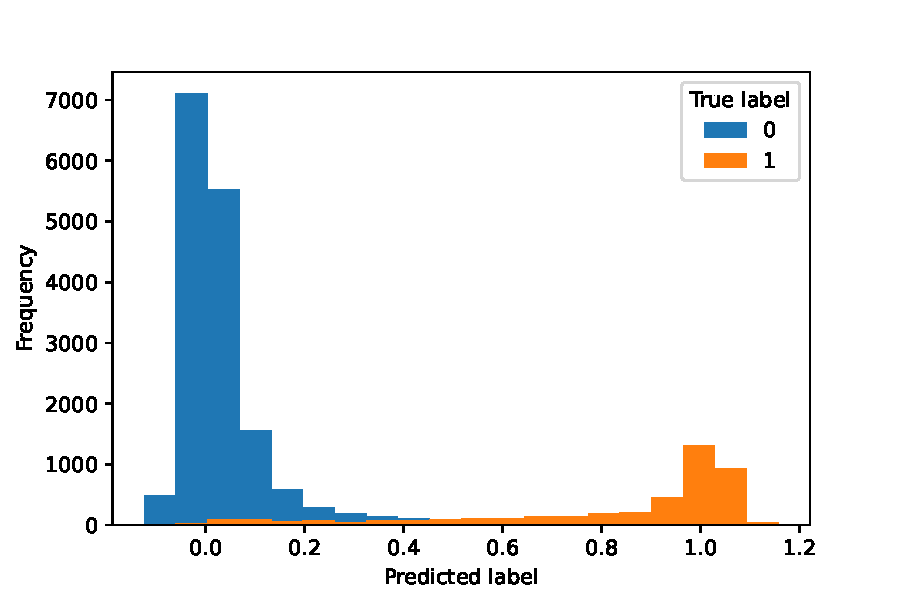
\includegraphics[width=\linewidth]{histogram-labels-bert-train.pdf}
        \vspace*{-3ex}
        \subcaption{Predictions with \BertBase on the training set.}
        \label{subfig:bert_train}
    \end{subfigure}
    \hfill
    \begin{subfigure}{0.49\linewidth}
        \vspace*{-1ex}
        \centering
        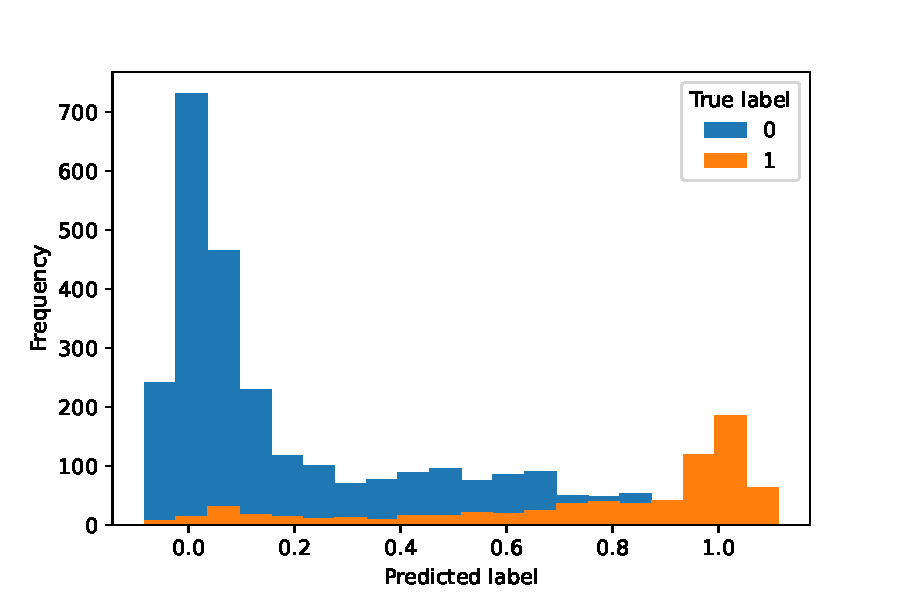
\includegraphics[width=\linewidth]{histogram-labels-bert-dev.pdf}
        \vspace*{-3ex}
        \subcaption{Predictions with \BertBase on the validation set.}
        \label{subfig:bert_dev}
    \end{subfigure}
    \begin{subfigure}{0.49\linewidth}
        \vspace*{-1ex}
        \centering
        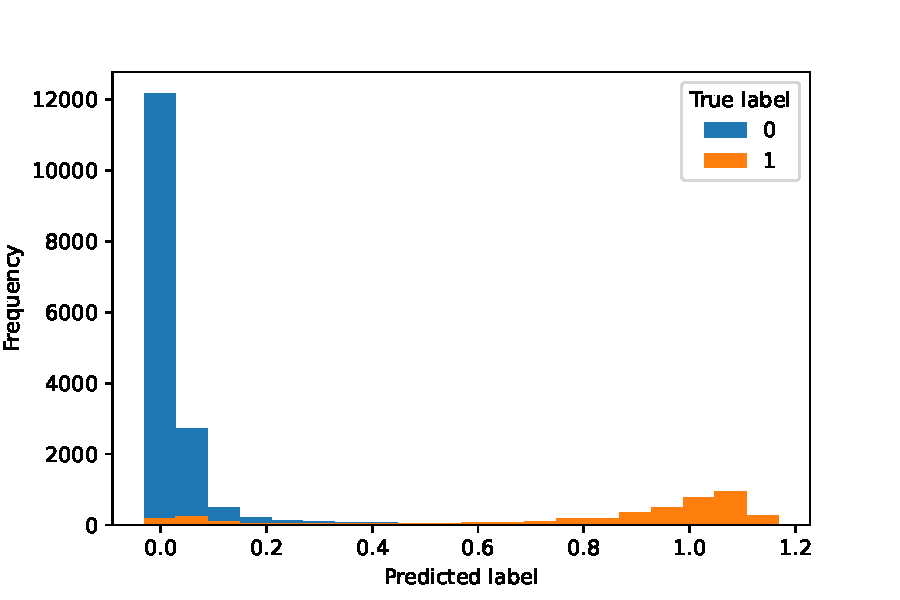
\includegraphics[width=\linewidth]{histogram-labels-roberta-train.pdf}
        \vspace*{-3ex}
        \subcaption{Predictions with \RobertaBase on the training set.}
        \label{subfig:roberta_train}
    \end{subfigure}
    \hfill
    \begin{subfigure}{0.49\linewidth}
        \vspace*{-1ex}
        \centering
        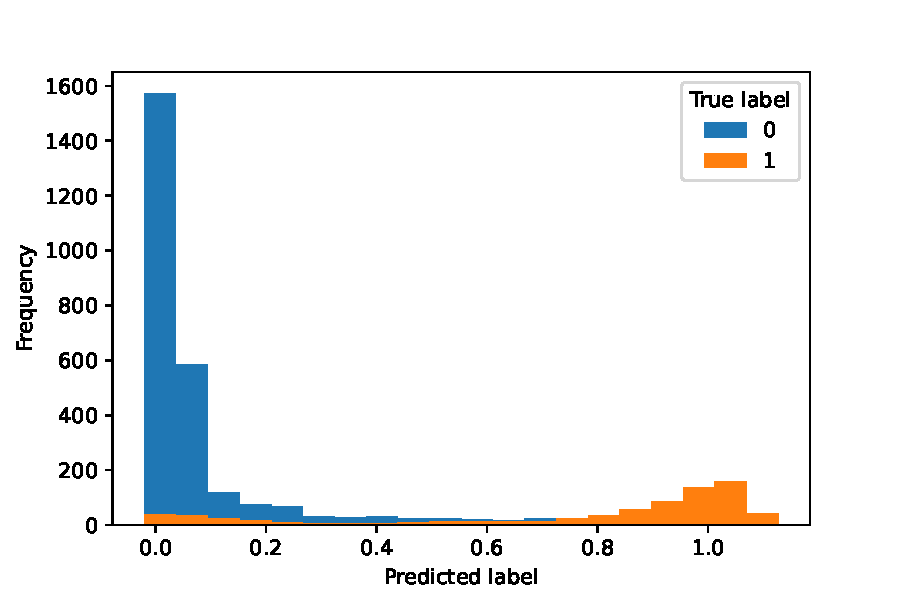
\includegraphics[width=\linewidth]{histogram-labels-roberta-dev.pdf}
        \vspace*{-3ex}
        \subcaption{Predictions with \RobertaBase on the validation set.}
        \label{subfig:roberta_dev}
    \end{subfigure}
    \caption{Histograms of predicted labels on the training and validation sets for argument key point pairs with the \BertBase and \RobertaBase classifiers. For good classifiers, predicted labels should approximately equal the true label~(0~or~1).}
    \label{fig:frequency}
\end{figure*}

\begin{table*}
    \caption{Examples of argument key point pairs from the \ArgKP dataset~\cite{Bar-HaimEFKLS2020} where the predicted score is off the ground truth label~(True) with either the \BertBase or \RobertaBase matcher.}
    \label{error-examples}
    \begin{tabularx}{\linewidth}{lXp{2.5cm}ccc}
      \toprule
      \textbf{\#} & \textbf{Argument} & \textbf{Key point} & \textbf{True} & \textbf{\Bert} & \textbf{\Roberta} \\
      \midrule
      D & % from validation set
      School uniforms can be less comfortable than students' regular clothes. & % arg_4_162
      School uniforms are expensive & % kp_4_6
      0 & \phantom{-}0.48 & 0.03 \\
      E & % from validation set
      affirmative action discriminates the majority, preventing skilled workers from gaining employment over someone less qualified but considered to be a member of a protected minority group. & % arg_15_113
      Affirmative action reduces quality & % kp_15_7
      1 & -0.05 & 0.03 \\
      % F & % from validation set
      % affirmative action can lead to people who are less qualified getting positions they would otherwise not be able to achieve, & % arg_15_110
      % Affirmative action reduces quality & % kp_15_7
      % 1 & -0.04 & 0.01 \\
      \bottomrule
    \end{tabularx}
  \end{table*}
  
\begin{figure}
    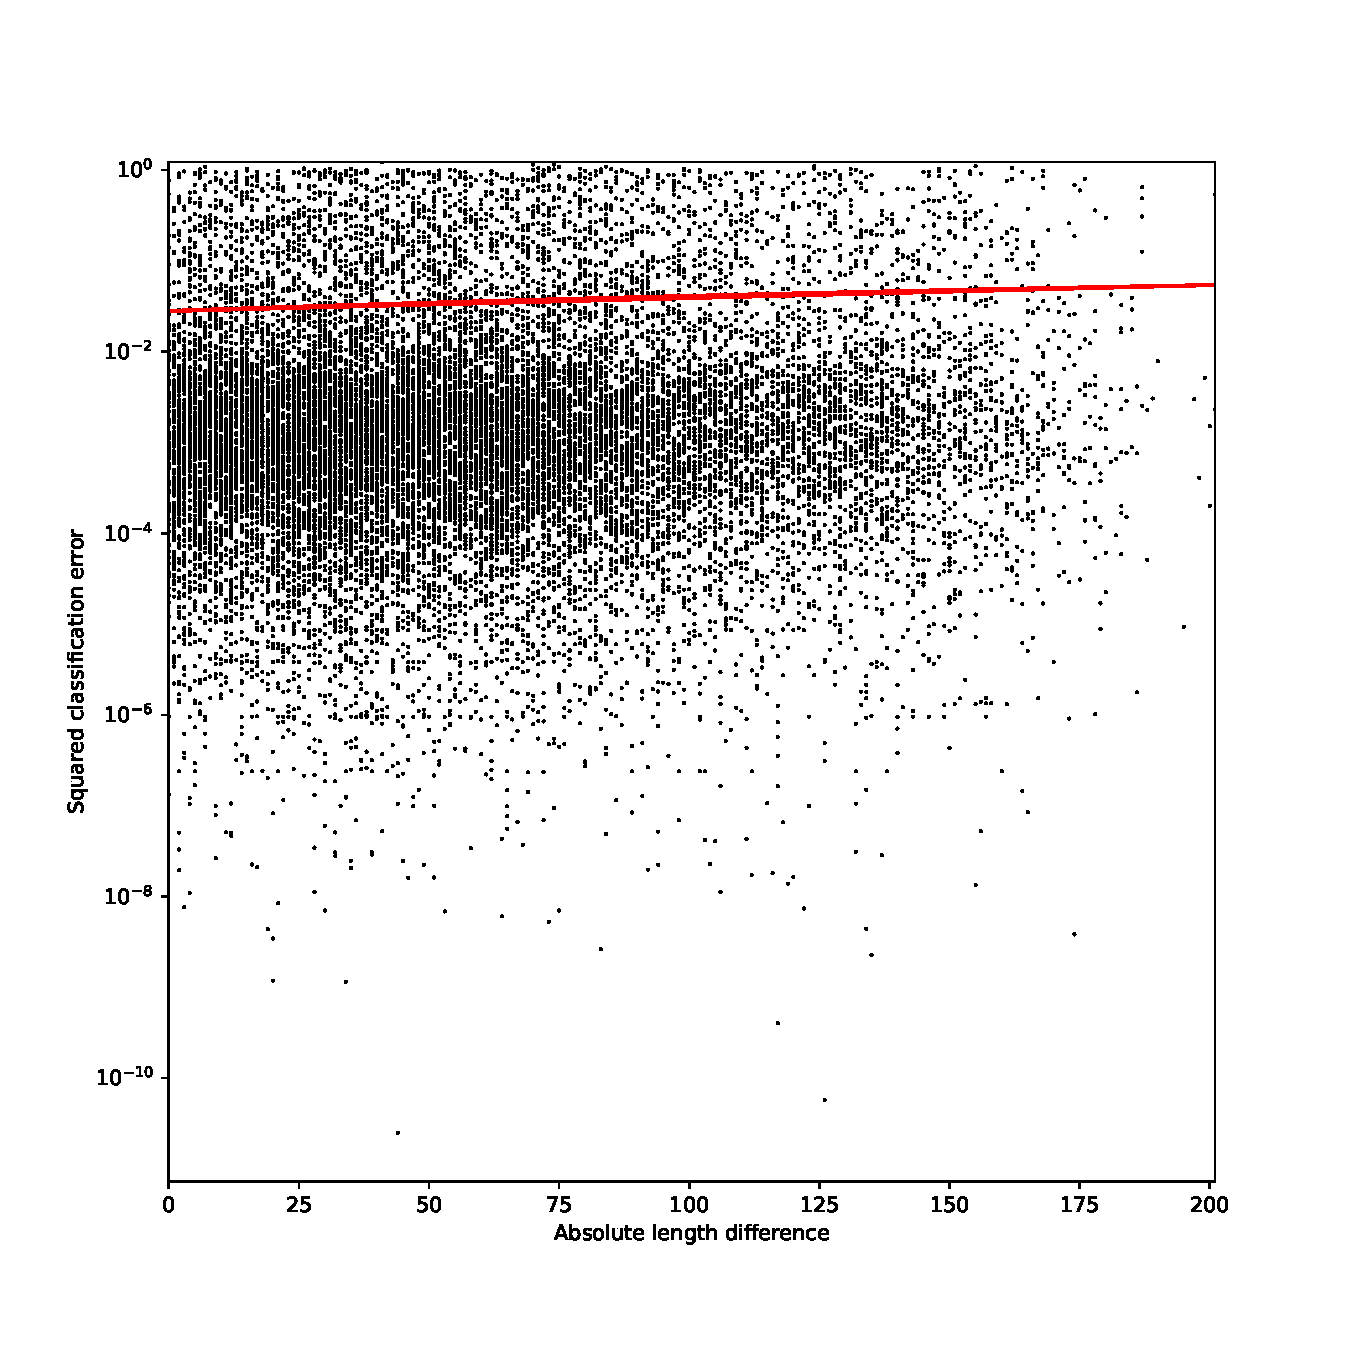
\includegraphics[width=\linewidth]{classification-error-length-difference-bert-train.pdf}
    \vspace*{-5ex}
    \caption{Squared classification error and absolute length difference between in characters each argument and key point pair from the validation set with the \BertBase matcher. The red line indicates the least squares polynomial fit.}
    \label{classification-error-length}
\end{figure}


To find errors in the two trained matchers, \BertBase and \RobertaBase, in Figure~\ref{fig:frequency} we show 
histograms of predicted match scores with respect to ground-truth labels.
Both matchers classify most pairs correctly, which can be seen because the histogram spikes around~0 for the 
true no-match label and around~1 for the true match label.
We also observe that predictions on the training set are closer to the true label than on the development set 
for both \RobertaBase and \BertBase.
Even though we expect any machine-learned matcher to perform better on training data than on validation data, 
we see this as a room for improvement with better generalization.
We notice that in Figures~\ref{subfig:bert_train} and~\ref{subfig:roberta_train} both approaches predict non-matching 
argument key point pairs better than matching key points.
This effect is likely to occur because of the higher amount of non-matching pairs provided.
Most arguments match with only a few or even just a single key point.
But nonetheless each argument is compared to all other key points, hence the underlying data to learn from is 
imbalanced~\cite{BarandelaVSF2004}.
Though, experiments with using textual data augmentation or simple oversampling to balance the dataset were 
unsuccessful~\cite{Dietterich1995}.
More advanced oversampling or undersampling approaches could possibly resolve this issue.
We further identify, that for matching arguments and key points, predicted scores from \BertBase are spread a 
bit more than scores from \RobertaBase.

In Figure~\ref{subfig:bert_dev}, we observe that the \BertBase matcher falsely predicts certain non-matching pairs with scores around~0.5.
An example of such uncertain pair is the argument key point pair~D from Table~\ref{error-examples}.
One reason we identify is that this argument has no matching key points given in the training dataset.
Hence, it is plausible that the \BertBase matcher has not learned well how to classify matches for that type of 
argument, and therefore predicts a neutral score of~\(0.48\).
The \RobertaBase matcher does not make that error, presumably because during pretraining \Roberta was given much 
more general-purpose information to infer from.

Both, the \BertBase matcher, but also \RobertaBase, falsely predict some argument key point pairs as non-matching that are in 
fact labelled as a match.
For example, it seems to be difficult to predict a match for the argument key point pair~E from Table~\ref{error-examples}.
The argument from the example is longer than most arguments and especially much longer than the key point~(431\,\%~more characters).
It might be more challenging to reduce such longer arguments, that contain more complex information, to very compact key points.
We confirm that observation by comparing the squared classification error with respect to the absolute difference between 
argument and key point lengths.
Figure~\ref{classification-error-length} shows a tendency of higher error with the \BertBase when the length difference 
between the argument and key point is large.
Comparable results can be observed for the \RobertaBase matcher.
We therefore identify length difference as a second general problem for both approaches.
